\usetikzlibrary{
  arrows.meta,
  backgrounds,
  calc,
  decorations.pathreplacing,
  fit,
  matrix,
  patterns.meta,
  positioning,
  shapes.geometric
}
\pgfplotsset{compat=1.18}

\definecolor{Ink}{HTML}{171717}
\definecolor{MutedInk}{HTML}{555555}
\definecolor{RuleGray}{HTML}{B8B8B8}
\definecolor{SoftGray}{HTML}{F2F2F0}
\definecolor{PanelGray}{HTML}{FAFAF8}
\definecolor{AccentBlue}{HTML}{1F4E79}
\definecolor{AccentGold}{HTML}{9A6B16}
\definecolor{AccentRed}{HTML}{8F2D2D}
\definecolor{AccentGreen}{HTML}{356B48}

\tikzset{
  paper box/.style={
    draw=Ink,
    rounded corners=2.5pt,
    line width=0.45pt,
    fill=white,
    align=center,
    inner sep=5pt,
    font=\sffamily\small
  },
  paper softbox/.style={
    paper box,
    fill=SoftGray
  },
  paper note/.style={
    draw=RuleGray,
    rounded corners=2pt,
    fill=PanelGray,
    align=left,
    inner sep=5pt,
    font=\sffamily\footnotesize
  },
  paper arrow/.style={
    -{Stealth[length=2.2mm]},
    line width=0.55pt,
    draw=Ink
  },
  paper dashed/.style={
    paper arrow,
    dashed,
    draw=MutedInk
  }
}

\newcommand{\scoreDots}[1]{%
  \ifcase#1\relax
  \or \textbullet\hspace{0.12em}{\color{RuleGray}\textbullet\textbullet}%
  \or \textbullet\textbullet\hspace{0.12em}{\color{RuleGray}\textbullet}%
  \or \textbullet\textbullet\textbullet%
  \fi
}

\newcommand{\figureContextAtGlance}{%
\begin{figure}[H]
\centering
\resizebox{\linewidth}{!}{%
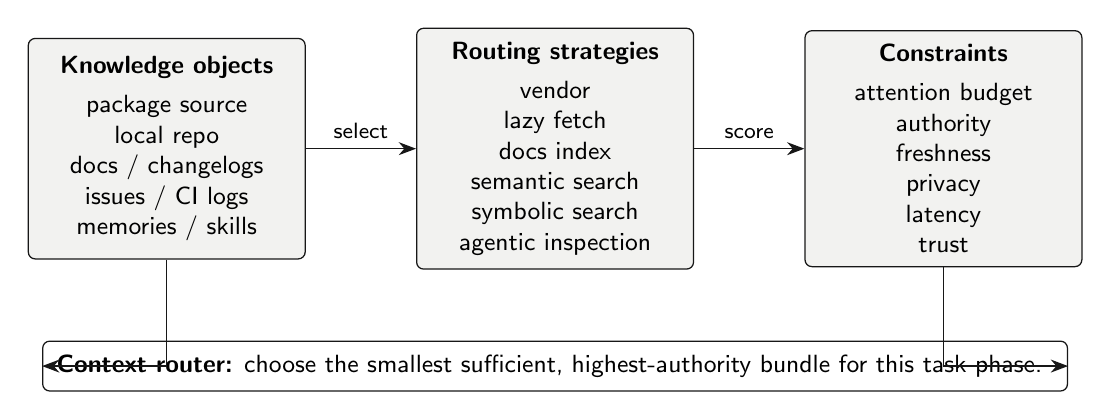
\begin{tikzpicture}[font=\sffamily, node distance=8mm]
  \node[paper softbox, minimum width=0.29\linewidth, minimum height=2.8cm] (objects) {
    \textbf{Knowledge objects}\\[3pt]
    package source\\
    local repo\\
    docs / changelogs\\
    issues / CI logs\\
    memories / skills
  };
  \node[paper softbox, right=14mm of objects, minimum width=0.29\linewidth, minimum height=2.8cm] (routes) {
    \textbf{Routing strategies}\\[3pt]
    vendor\\
    lazy fetch\\
    docs index\\
    semantic search\\
    symbolic search\\
    agentic inspection
  };
  \node[paper softbox, right=14mm of routes, minimum width=0.29\linewidth, minimum height=2.8cm] (constraints) {
    \textbf{Constraints}\\[3pt]
    attention budget\\
    authority\\
    freshness\\
    privacy\\
    latency\\
    trust
  };

  \draw[paper arrow] (objects) -- node[above, font=\sffamily\footnotesize] {select} (routes);
  \draw[paper arrow] (routes) -- node[above, font=\sffamily\footnotesize] {score} (constraints);
  \node[paper box, below=9mm of routes, minimum width=0.78\linewidth] (policy) {
    \textbf{Context router:} choose the smallest sufficient, highest-authority bundle for this task phase.
  };
  \draw[paper arrow] (constraints.south) |- (policy.east);
  \draw[paper arrow] (objects.south) |- (policy.west);
\end{tikzpicture}
}
\caption{Context routing at a glance. The paper's thesis is not that one context source wins; it is that coding agents need an explicit allocation policy over objects, routes, and constraints.}
\label{fig-context-at-glance}
\end{figure}
}

\newcommand{\figureUtilityTradeoff}{%
\begin{figure}[H]
\centering
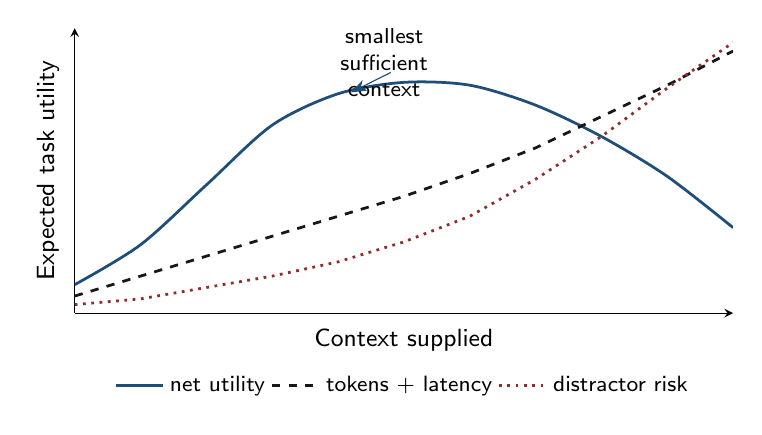
\begin{tikzpicture}
\begin{axis}[
  width=0.82\linewidth,
  height=5.2cm,
  axis lines=left,
  xlabel={Context supplied},
  ylabel={Expected task utility},
  xmin=0, xmax=10,
  ymin=0, ymax=10,
  xtick=\empty,
  ytick=\empty,
  legend style={draw=none, fill=none, at={(0.5,-0.18)}, anchor=north, legend columns=3, font=\sffamily\footnotesize},
  every axis plot/.append style={line width=1pt},
  label style={font=\sffamily\small},
]
\addplot[AccentBlue, mark=none, smooth] coordinates {(0,1.0) (1,2.4) (2,4.5) (3,6.6) (4,7.7) (5,8.1) (6,8.0) (7,7.3) (8,6.2) (9,4.8) (10,3.0)};
\addlegendentry{net utility}
\addplot[Ink, dashed, mark=none] coordinates {(0,0.6) (1,1.3) (2,2.0) (3,2.7) (4,3.4) (5,4.1) (6,4.9) (7,5.8) (8,6.9) (9,8.0) (10,9.2)};
\addlegendentry{tokens + latency}
\addplot[AccentRed, dotted, mark=none] coordinates {(0,0.3) (1,0.5) (2,0.9) (3,1.3) (4,1.8) (5,2.5) (6,3.4) (7,4.7) (8,6.2) (9,7.9) (10,9.5)};
\addlegendentry{distractor risk}
\node[font=\sffamily\footnotesize, align=center] at (axis cs:4.7,8.8) {smallest\\sufficient\\context};
\draw[-{Stealth[length=2mm]}, AccentBlue] (axis cs:4.8,8.45) -- (axis cs:4.2,7.75);
\end{axis}
\end{tikzpicture}
\caption{The router optimizes expected utility, not raw context size. More context helps until authority and relevance are outweighed by token, latency, staleness, trust, and distractor costs.}
\label{fig-utility-tradeoff}
\end{figure}
}

\newcommand{\figureLongContextDegradation}{%
\begin{figure}[H]
\centering
\begin{tikzpicture}
\begin{groupplot}[
  group style={group size=2 by 1, horizontal sep=1.2cm},
  width=0.46\linewidth,
  height=5.3cm,
  ymin=0,
  ymax=80,
  ymajorgrids=true,
  grid style={draw=RuleGray!45},
  ylabel={Success / score (\%)},
  label style={font=\sffamily\small},
  tick label style={font=\sffamily\footnotesize},
  title style={font=\sffamily\small\bfseries},
  nodes near coords,
  every node near coord/.append style={font=\sffamily\scriptsize, yshift=2pt},
]
\nextgroupplot[
  title={LongSWE-Bench},
  symbolic x coords={32K,256K},
  xtick=data,
]
\addplot[AccentBlue, mark=*, line width=1pt] coordinates {(32K,29) (256K,3)};
\nextgroupplot[
  title={LongCodeQA},
  symbolic x coords={512K,1M},
  xtick=data,
]
\addplot[AccentGold, mark=square*, line width=1pt] coordinates {(512K,70.2) (1M,40.0)};
\end{groupplot}
\end{tikzpicture}
\caption{LongCodeBench examples used in this paper. Claude 3.5 Sonnet drops on LongSWE-Bench from 29\% at 32K to 3\% at 256K; Qwen2.5 drops on LongCodeQA from 70.2\% at 512K to 40.0\% at 1M. The point is calibration, not a universal threshold.}
\label{fig-longcodebench}
\end{figure}
}

\newcommand{\figureRetrievalLandscape}{%
\begin{figure}[H]
\centering
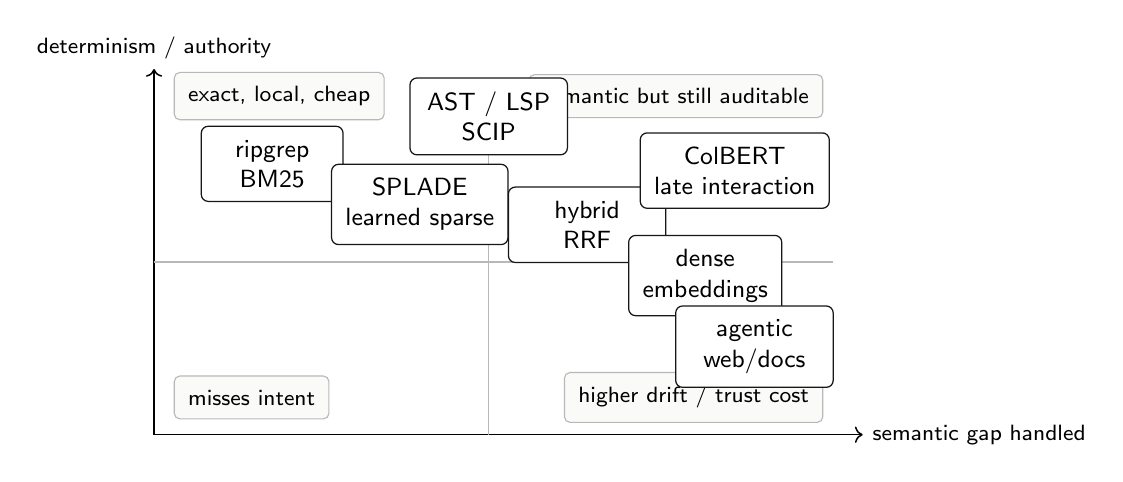
\begin{tikzpicture}[x=1.25cm, y=0.86cm, font=\sffamily\footnotesize]
  \draw[->, line width=0.55pt] (0,0) -- (7.2,0) node[right] {semantic gap handled};
  \draw[->, line width=0.55pt] (0,0) -- (0,5.4) node[above] {determinism / authority};
  \draw[RuleGray] (3.4,0) -- (3.4,5.1);
  \draw[RuleGray] (0,2.55) -- (6.9,2.55);

  \node[paper note, anchor=west] at (0.2,5.0) {exact, local, cheap};
  \node[paper note, anchor=east] at (6.8,5.0) {semantic but still auditable};
  \node[paper note, anchor=west] at (0.2,0.55) {misses intent};
  \node[paper note, anchor=east] at (6.8,0.55) {higher drift / trust cost};

  \node[paper box, minimum width=1.8cm] at (1.2,4.0) {ripgrep\\BM25};
  \node[paper box, minimum width=2.1cm] at (2.7,3.4) {SPLADE\\learned sparse};
  \node[paper box, minimum width=2.0cm] at (4.4,3.1) {hybrid\\RRF};
  \node[paper box, minimum width=1.9cm] at (5.6,2.35) {dense\\embeddings};
  \node[paper box, minimum width=1.9cm] at (5.9,3.9) {ColBERT\\late interaction};
  \node[paper box, minimum width=2.0cm] at (3.4,4.7) {AST / LSP\\SCIP};
  \node[paper box, minimum width=2.0cm] at (6.1,1.3) {agentic\\web/docs};
\end{tikzpicture}
\caption{Semantic and non-semantic search are complements. Exact lexical search is cheap and deterministic; dense and late-interaction search bridge intent gaps; graph and symbol search preserve code authority; hybrid retrieval is often the pragmatic route.}
\label{fig-retrieval-landscape}
\end{figure}
}

\newcommand{\figureFailureModes}{%
\begin{figure}[H]
\centering
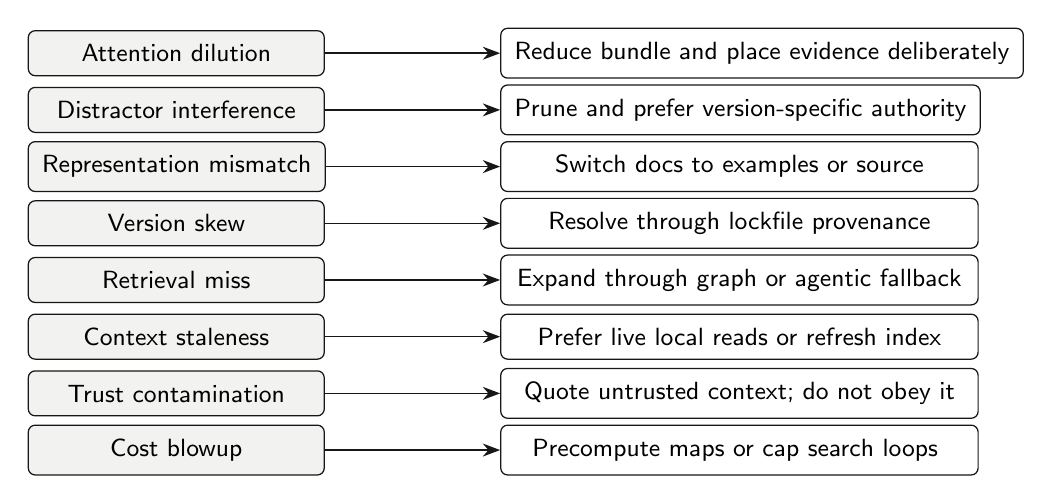
\begin{tikzpicture}[font=\sffamily\footnotesize, node distance=3.5mm]
  \foreach \i/\failure/\response in {
    0/Attention dilution/Reduce bundle and place evidence deliberately,
    1/Distractor interference/Prune and prefer version-specific authority,
    2/Representation mismatch/Switch docs to examples or source,
    3/Version skew/Resolve through lockfile provenance,
    4/Retrieval miss/Expand through graph or agentic fallback,
    5/Context staleness/Prefer live local reads or refresh index,
    6/Trust contamination/Quote untrusted context; do not obey it,
    7/Cost blowup/Precompute maps or cap search loops
  }{
    \pgfmathsetmacro{\y}{-\i*0.72}
    \node[paper softbox, minimum width=0.31\linewidth, anchor=west] (f\i) at (0,\y) {\failure};
    \node[paper box, minimum width=0.50\linewidth, anchor=west] (r\i) at (6.0,\y) {\response};
    \draw[paper arrow] (f\i.east) -- (r\i.west);
  }
\end{tikzpicture}
\caption{Wrong context has concrete failure modes. A router is useful only if each failure maps to an intervention: prune, switch representation, refresh, change authority, or stop searching.}
\label{fig-failure-modes}
\end{figure}
}

\newcommand{\heatcell}[1]{%
  \ifcase#1\cellcolor{white}0%
  \or\cellcolor{SoftGray}1%
  \or\cellcolor{RuleGray!45}2%
  \or\cellcolor{Ink!72}\textcolor{white}{3}%
  \fi
}

\newcommand{\figurePhaseHeatmap}{%
\begin{figure}[H]
\centering
\small
\setlength{\tabcolsep}{4pt}
\renewcommand{\arraystretch}{1.12}
\begin{tabular}{lcccccc}
\toprule
\textbf{Phase} & \rotatebox{45}{Rules} & \rotatebox{45}{Repo map} & \rotatebox{45}{Search} & \rotatebox{45}{Files} & \rotatebox{45}{Package src} & \rotatebox{45}{Tests/logs}\\
\midrule
Orient    & \heatcell{3} & \heatcell{3} & \heatcell{1} & \heatcell{1} & \heatcell{0} & \heatcell{0}\\
Locate    & \heatcell{1} & \heatcell{2} & \heatcell{3} & \heatcell{2} & \heatcell{1} & \heatcell{1}\\
Plan      & \heatcell{2} & \heatcell{1} & \heatcell{2} & \heatcell{3} & \heatcell{2} & \heatcell{1}\\
Edit      & \heatcell{1} & \heatcell{0} & \heatcell{1} & \heatcell{3} & \heatcell{2} & \heatcell{1}\\
Verify    & \heatcell{1} & \heatcell{0} & \heatcell{1} & \heatcell{2} & \heatcell{1} & \heatcell{3}\\
Repair    & \heatcell{1} & \heatcell{1} & \heatcell{3} & \heatcell{3} & \heatcell{3} & \heatcell{3}\\
Summarize & \heatcell{2} & \heatcell{2} & \heatcell{0} & \heatcell{2} & \heatcell{0} & \heatcell{1}\\
\bottomrule
\end{tabular}
\caption{Task-phase context heatmap. Darker cells indicate higher expected usefulness. Context routing is an online policy: the right bundle changes as the agent orients, locates, edits, verifies, repairs, and summarizes.}
\label{fig-phase-heatmap}
\end{figure}
}

\newcommand{\figureRouterArchitecture}{%
\begin{figure}[H]
\centering
\resizebox{\linewidth}{!}{%
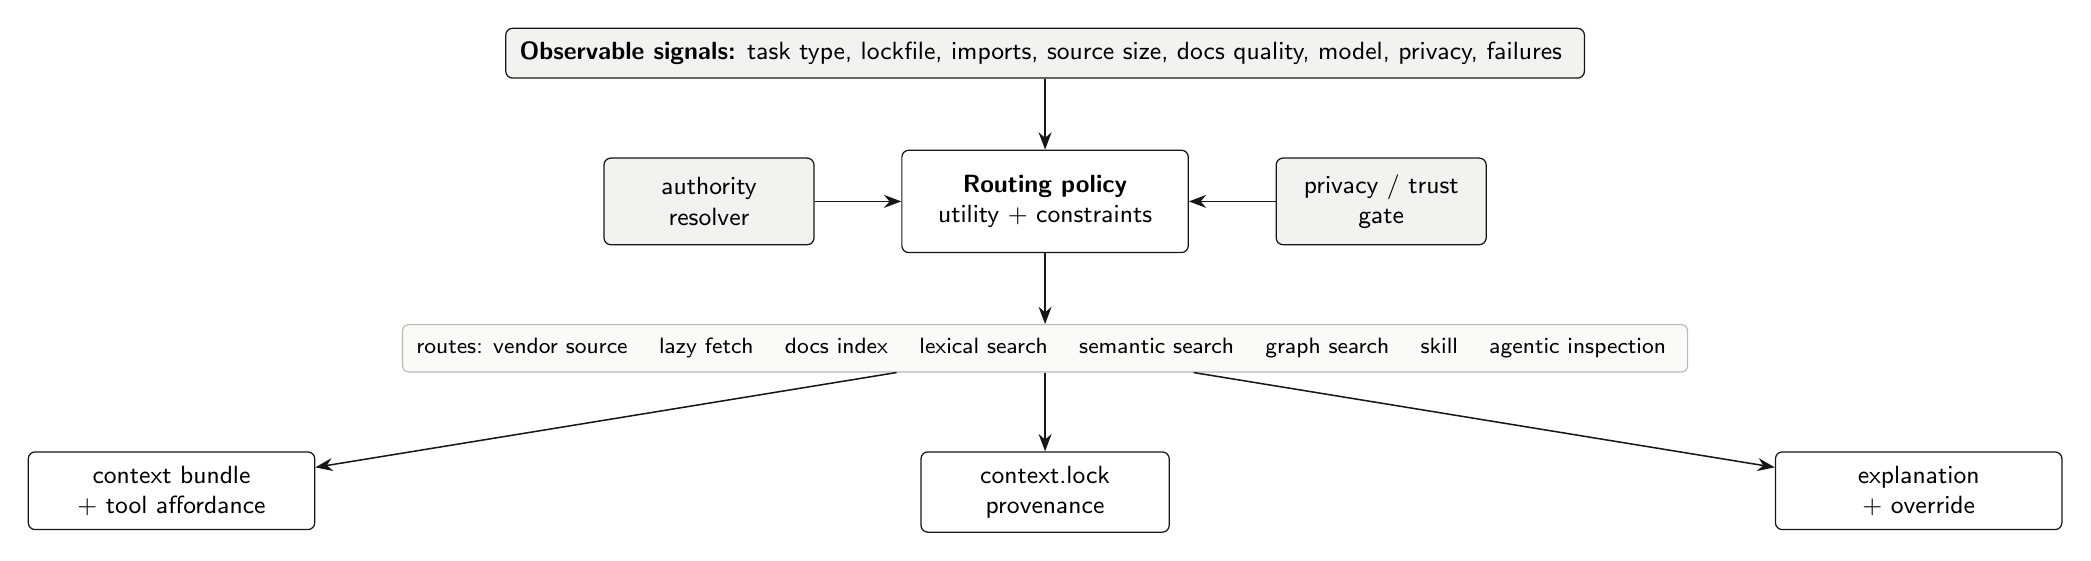
\begin{tikzpicture}[font=\sffamily\footnotesize, node distance=7mm]
  \node[paper softbox, minimum width=0.86\linewidth] (signals) {
    \textbf{Observable signals:} task type, lockfile, imports, source size, docs quality, model, privacy, failures
  };
  \node[paper box, below=9mm of signals, minimum width=0.30\linewidth, minimum height=1.3cm] (policy) {\textbf{Routing policy}\\utility + constraints};
  \node[paper softbox, left=11mm of policy, minimum width=0.22\linewidth, minimum height=1.1cm] (authority) {authority\\resolver};
  \node[paper softbox, right=11mm of policy, minimum width=0.22\linewidth, minimum height=1.1cm] (trust) {privacy / trust\\gate};
  \node[paper note, below=9mm of policy, minimum width=0.78\linewidth] (routes) {
    routes: vendor source \quad lazy fetch \quad docs index \quad lexical search \quad semantic search \quad graph search \quad skill \quad agentic inspection
  };
  \node[paper box, below left=10mm and 11mm of routes, minimum width=0.30\linewidth] (bundle) {context bundle\\+ tool affordance};
  \node[paper box, below=10mm of routes, minimum width=0.26\linewidth] (lock) {context.lock\\provenance};
  \node[paper box, below right=10mm and 11mm of routes, minimum width=0.30\linewidth] (explain) {explanation\\+ override};

  \draw[paper arrow] (signals) -- (policy);
  \draw[paper arrow] (authority) -- (policy);
  \draw[paper arrow] (trust) -- (policy);
  \draw[paper arrow] (policy) -- (routes);
  \draw[paper arrow] (routes) -- (bundle);
  \draw[paper arrow] (routes) -- (lock);
  \draw[paper arrow] (routes) -- (explain);
\end{tikzpicture}
}
\caption{Context router architecture redrawn as a PDF-native diagram. The router does not merely retrieve content; it resolves authority, enforces trust policy, emits provenance, and explains the route.}
\label{fig-router}
\end{figure}
}

\newcommand{\figureVercelEval}{%
\begin{figure}[H]
\centering
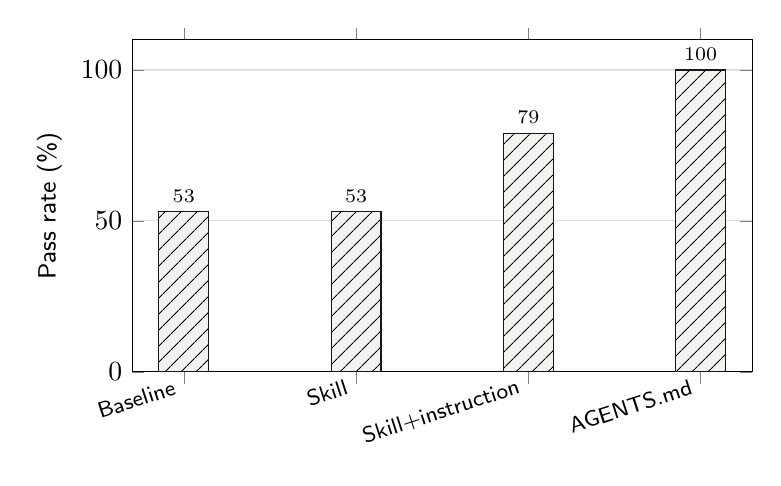
\begin{tikzpicture}
\begin{axis}[
  ybar,
  width=0.78\linewidth,
  height=5.8cm,
  ymin=0,
  ymax=110,
  ylabel={Pass rate (\%)},
  symbolic x coords={Baseline,Skill,Skill+instruction,AGENTS.md},
  xtick=data,
  x tick label style={rotate=18, anchor=east, font=\sffamily\footnotesize},
  ymajorgrids=true,
  grid style={draw=RuleGray!45},
  bar width=18pt,
  nodes near coords,
  every node near coord/.append style={font=\sffamily\scriptsize},
  label style={font=\sffamily\small},
]
\addplot[draw=Ink, fill=SoftGray, postaction={pattern={Lines[angle=45,distance=4pt,line width=0.35pt]}}] coordinates {
  (Baseline,53) (Skill,53) (Skill+instruction,79) (AGENTS.md,100)
};
\end{axis}
\end{tikzpicture}
\caption{Vercel's reported Next.js agent eval results. The lesson for routing is selector and timing: an always-on compact docs index outperformed an on-demand skill in this suite.}
\label{fig-vercel-eval}
\end{figure}
}

\newcommand{\figureEvalLattice}{%
\begin{figure}[H]
\centering
\scriptsize
\setlength{\tabcolsep}{3.2pt}
\renewcommand{\arraystretch}{1.12}
\begin{tabular}{lcccccccc}
\toprule
\textbf{Strategy} & \rotatebox{45}{Unknown lib} & \rotatebox{45}{Framework idiom} & \rotatebox{45}{Migration} & \rotatebox{45}{Stack trace} & \rotatebox{45}{Multi-file} & \rotatebox{45}{Security} & \rotatebox{45}{Perf/debug} & \rotatebox{45}{Test repair}\\
\midrule
No extra context       & -- & -- & -- & -- & o  & o  & -- & o  \\
Docs-only              & +  & o  & +  & -- & -- & +  & -- & o  \\
Always-on docs index   & +  & +  & +  & o  & o  & +  & -- & o  \\
Source vendoring       & o  & +  & o  & +  & o  & o  & +  & +  \\
Lazy source fetch      & o  & o  & o  & +  & o  & o  & +  & +  \\
Repo pack              & o  & o  & -- & o  & +  & -- & o  & o  \\
Semantic index         & +  & o  & o  & o  & +  & o  & o  & o  \\
Structural index       & o  & +  & o  & +  & +  & o  & +  & +  \\
Agentic search         & o  & +  & o  & +  & +  & o  & +  & +  \\
Router                 & +  & +  & +  & +  & +  & +  & +  & +  \\
\bottomrule
\end{tabular}
\caption{Evaluation lattice. Symbols encode expected route relevance: `+' core condition, `o' optional condition, `--' weak or negative-control condition. A router benchmark should vary strategy while holding agent and task fixed.}
\label{fig-eval-lattice}
\end{figure}
}

\newcommand{\figureToolLandscapeCounts}{%
\begin{figure}[H]
\centering
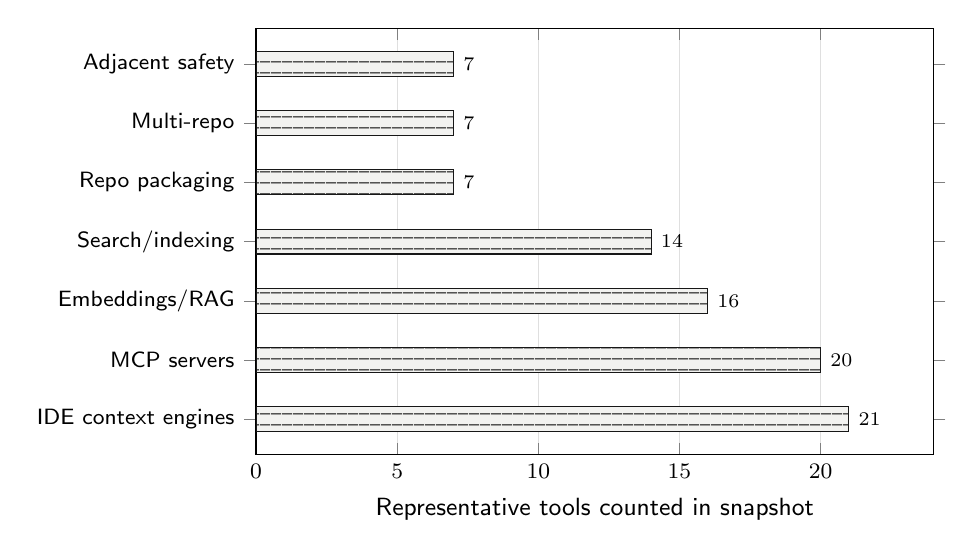
\begin{tikzpicture}
\begin{axis}[
  xbar,
  width=0.84\linewidth,
  height=7.0cm,
  xmin=0,
  xmax=24,
  xlabel={Representative tools counted in snapshot},
  symbolic y coords={Adjacent safety,Multi-repo,Repo packaging,Search/indexing,Embeddings/RAG,MCP servers,IDE context engines},
  ytick=data,
  y dir=reverse,
  nodes near coords,
  every node near coord/.append style={font=\sffamily\scriptsize},
  tick label style={font=\sffamily\footnotesize},
  label style={font=\sffamily\small},
  xmajorgrids=true,
  grid style={draw=RuleGray!45},
  bar width=9pt,
]
\addplot[draw=Ink, fill=SoftGray, postaction={pattern={Lines[angle=0,distance=4pt,line width=0.35pt]}}] coordinates {
  (7,Adjacent safety)
  (7,Multi-repo)
  (7,Repo packaging)
  (14,Search/indexing)
  (16,Embeddings/RAG)
  (20,MCP servers)
  (21,IDE context engines)
};
\end{axis}
\end{tikzpicture}
\caption{Tool-landscape fragmentation in the May 2026 snapshot. The distribution itself motivates routing: tools cluster around different context surfaces rather than one universal context strategy.}
\label{fig-tool-counts}
\end{figure}
}
